\section{Auswertung}
\label{sec:Auswertung}
Ziel der Auswertung ist das Bestimmen der Spaltbreite $b_i$ und ein anschließender Vergleich mit der Herstellerangabe.
Für den Versuch werden alle zur Verfügung stehenden Randdaten dokumentiert.

\begin{table}
    \centering
    \caption{Kenndaten der Versuchsdurchführung.}
    \begin{tabular}{c c c c c c c}
        \toprule
        & $s\:/\:\si{\milli\meter}$ & $b_i\:/\:\si{\milli\meter}$ & $\lambda\:/\:\si{\nano\meter}$ & $d\:/\:\si{\milli\meter}$ & $I_d\:/\:\si{\micro\ampere}$ \\
        \midrule
        Doppelspalt & 0.75 & 0.150 & 633 & 626.1 & 0.63 \\
        Einzelspalt &      & 0.075 & 633 & 626.1 & 0.70 \\
        \bottomrule
    \end{tabular}
\end{table}

\subsection{Einzelspalt}

\begin{table}
    \centering
    \caption{Messwerte zum Einzelspalt.}
    \label{tab:Mess1}
    \begin{tabular}{S[table-format=1.1] S[table-format=1.3] S[table-format=2.2] S[table-format=1.1] S[table-format=1.3] S[table-format=2.2] S[table-format=1.1] S[table-format=1.3]}
        \toprule
        $x\:/\:\si{\milli\meter}$ & $I\:/\:\si{\micro\ampere}$ &&
        $x\:/\:\si{\milli\meter}$ & $I\:/\:\si{\micro\ampere}$ &&
        $x\:/\:\si{\milli\meter}$ & $I\:/\:\si{\micro\ampere}$ \\
        \midrule
        0.0 & 0.880 && 8.5   & 3.300  && 17.0 & 0.865 \\
        0.5 & 0.840 && 9.0   & 5.000  && 17.5 & 0.990 \\
        1.0 & 0.778 && 9.5   & 7.000  && 18.0 & 1.150 \\
        1.5 & 0.740 && 10.0  & 9.000  && 18.5 & 1.260 \\
        2.0 & 0.758 && 10.5  & 10.700 && 19.0 & 1.290 \\
        2.5 & 0.854 && 11.0  & 12.100 && 19.5 & 1.220 \\
        3.0 & 1.000 && 11.5  & 12.700 && 20.0 & 1.100 \\
        3.5 & 1.200 && 12.0  & 12.700 && 20.5 & 0.975 \\
        4.0 & 1.340 && 12.5  & 12.250 && 21.0 & 0.880 \\
        4.5 & 1.430 && 13.0  & 10.600 && 21.5 & 0.842 \\
        5.0 & 1.400 && 13.5  & 8.850  && 22.0 & 0.879 \\
        5.5 & 1.250 && 14.0  & 6.790  && 22.5 & 0.945 \\
        6.0 & 1.050 && 14.5  & 4.780  && 23.0 & 1.000 \\
        6.5 & 0.900 && 15.0  & 3.000  && 23.5 & 1.060 \\
        7.0 & 0.910 && 15.5  & 1.920  && 24.0 & 1.070 \\
        7.5 & 1.260 && 16.0  & 1.200  && 24.5 & 1.025 \\
        8.0 & 2.040 && 16.5  & 0.890  &&      &       \\
        \bottomrule
    \end{tabular}
\end{table}

Für die Ausgleichskurve des Einzelspalts wird eine Funktion der Form
\begin{equation}
    I(\varphi) = (ab_{par, 1}\frac{\sin{\gamma}}{\gamma})^2 + c
\end{equation}
verwendet mit 
\begin{equation}
    \gamma = \frac{2\pi \sin\varphi}{\lambda}
    \label{eqn:gamma}
\end{equation}
\begin{equation}
    \sin\varphi = \frac{x'}{d'}
\end{equation}
\begin{equation}
    d' = \sqrt{d^2 + x'^2}
\end{equation}
und
\begin{equation}
    x' = |x - x_0| \:.
\end{equation}
Die variablen Parameter der Funktion sind $x_0$, $a$, $b_{par, 1}$, und $c$, wobei $x_0$ das Intensitätsmaximum, $a$ das $A_0$ aus \eqref{eqn:I}, $b_{par, 1}$ die Spaltbreite und $c$ der Dunkelstrom
$I_d$ ist.
Das fitten mit der Funktion mit \texttt{curve\_fit}\cite{scipy} liefert die Werte in Tabelle \ref{tab:parEinzel}.

\begin{table}
    \centering
    \caption{Parameterwerte des Einzelspalts.}
    \label{tab:parEinzel}
    \begin{tabular}{c S[table-format=1.4]@{\,\( \pm \)\,}S[table-format=1.4] 
        S[table-format=1.5]@{\,\( \pm \)\,}S[table-format=1.5] 
        S[table-format=1.2]@{\,\( \pm \)\,}S[table-format=1.2]
        S[table-format=1.3]@{\,\( \pm \)\,}S[table-format=1.3]}
        \toprule
        & \multicolumn{2}{c}{$a$} & \multicolumn{2}{c}{$b_{par, 1}\:/\:\si{\milli\meter}$} & \multicolumn{2}{c}{$c\:/\:\si{\micro\ampere}$} & \multicolumn{2}{c}{$x_0\:/\:\si{\milli\meter}$} \\
        \midrule
        Einzelspalt & 0.1395&0.0004 & 0.02495&0.00007 & 0.81&0.01 & 11.727&0.006 \\
    \end{tabular}
\end{table}
Verschiedene Formen der Funktion im Programmcode und verschiedene Startwerte für die Parameter liefern stets die gleichen Ergebnisse mit Abweichungen im Promille-Bereich.
Der Vergleich der Herstellerangabe mit dem errechneten Wert für die Spaltbreite ist um den Faktor 3 verschieden mit $b_{par, 1} \approx \SI{0.025}{\milli\meter}$
\begin{equation}
    \frac{b_{par, 1}}{b_1} = \frac{\SI{0.025}{\milli\meter}}{\SI{0.075}{\milli\meter}} = 3\:.
\end{equation}
Der relative Fehler von $b_{par, 1}$ ist $\approx 0.28\%$.

\begin{figure}
    \centering
    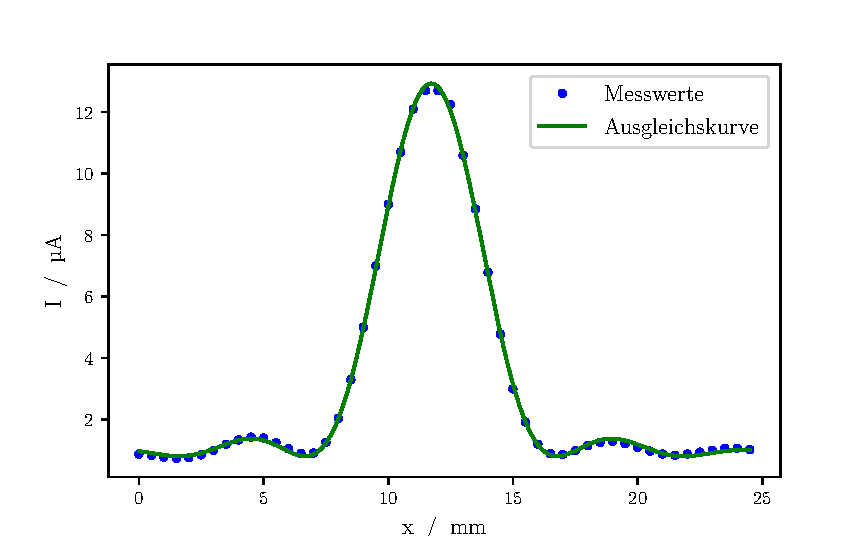
\includegraphics[width=.9\textwidth]{python/EinzelspaltFit.pdf}
    \caption{Messwerte und Ausgleichskurve zum Einzelspalt.}
    \label{fig:messEinzel}
\end{figure}

Der abgeschätzte Wert des Intensitätsmaximums $x_0$ liegt bei $\SI{11.727 \pm 0.006}{\milli\meter}$ mit einer Abweichung von $0.05\%$.

\subsection{Doppelspalt}
\begin{table}
    \centering
    \caption{Parameterwerte des Doppelspalts.}
    \label{tab:parDoppel}
    \begin{tabular}{c S[table-format=1.4]@{\,\( \pm \)\,}S[table-format=1.4] 
        S[table-format=1.5]@{\,\( \pm \)\,}S[table-format=1.5] 
        S[table-format=1.2]@{\,\( \pm \)\,}S[table-format=1.2]
        S[table-format=1.3]@{\,\( \pm \)\,}S[table-format=1.3]}
        \toprule
        & \multicolumn{2}{c}{$a$} & \multicolumn{2}{c}{$b_{par, 2}\:/\:\si{\milli\meter}$} & \multicolumn{2}{c}{$c\:/\:\si{\micro\ampere}$} & \multicolumn{2}{c}{$x_0\:/\:\si{\milli\meter}$} \\
        \midrule
        Doppelspalt & 0.1210&0.0006 & 0.0752&0.0004 & 0.38&0.12 & 11.077&0.006 \\
    \end{tabular}
\end{table}

\begin{table}
    \centering
        \caption{Messwerte zum Doppelspalt.}
        \label{tab:Mess2}
        \begin{tabular}{S[table-format=1.1] S[table-format=1.3] S[table-format=2.2] S[table-format=1.1] S[table-format=1.3] S[table-format=2.2] S[table-format=1.1] S[table-format=1.3]}
            \toprule
            $x\:/\:\si{\milli\meter}$ & $I\:/\:\si{\micro\ampere}$ &&
            $x\:/\:\si{\milli\meter}$ & $I\:/\:\si{\micro\ampere}$ &&
            $x\:/\:\si{\milli\meter}$ & $I\:/\:\si{\micro\ampere}$ \\
            \midrule
            0.00 & 0.942 && 7.99  & 2.420  && 15.98 & 0.800 \\
            0.47 & 0.920 && 8.46  & 1.300  && 16.45 & 0.960 \\
            0.94 & 0.718 && 8.93  & 4.350  && 16.92 & 1.380 \\
            1.41 & 0.620 && 9.40  & 15.800 && 17.39 & 1.430 \\
            1.88 & 0.724 && 9.87  & 42.400 && 17.86 & 1.030 \\
            2.35 & 0.910 && 10.34 & 63.000 && 18.33 & 0.710 \\
            2.82 & 0.936 && 10.81 & 80.000 && 18.80 & 0.730 \\
            3.29 & 0.750 && 11.28 & 81.800 && 19.27 & 0.940 \\
            3.76 & 0.635 && 11.75 & 67.500 && 19.74 & 1.050 \\
            4.23 & 0.810 && 12.22 & 42.500 && 20.21 & 0.840 \\
            4.70 & 1.120 && 12.69 & 20.400 && 20.68 & 0.665 \\
            5.17 & 1.140 && 13.16 & 6.350  && 21.15 & 0.685 \\
            5.64 & 1.070 && 13.63 & 1.430  && 21.62 & 0.855 \\
            6.11 & 0.720 && 14.10 & 1.880  && 22.09 & 0.980 \\
            6.58 & 1.445 && 14.57 & 2.950  && 22.56 & 0.900 \\
            7.05 & 2.850 && 15.04 & 2.740  && 23.03 & 0.715 \\
            7.52 & 3.450 && 15.51 & 1.540  &&       &       \\
            \bottomrule
        \end{tabular}
\end{table}

Für den Doppelspalt wird die angepasste Funktion \eqref{eqn:doppelspalt} verwendet. Dabei entspricht das $\gamma$ dem aus \eqref{eqn:gamma}.

Als Kontrollwert der Parameter für den Doppelspalt eignet sich $x_0 = \SI{11.077 \pm 0.006}{\milli\meter}$, welcher eine gute und plausible Annäherung an das gemessene Intensitätsmaximum ist. (Vgl. Tab. \ref{tab:Mess2} und Abb. \ref{fig:messDoppel})
\begin{figure}
    \centering
    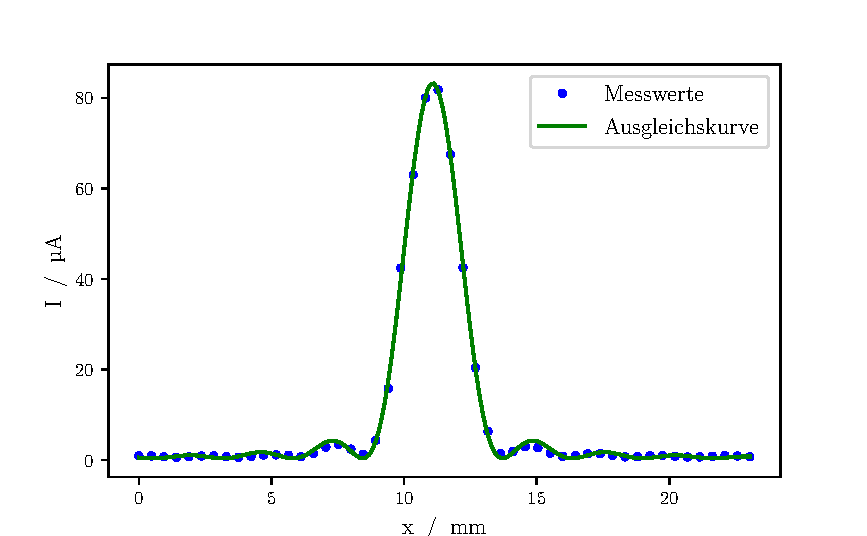
\includegraphics[width=.9\textwidth]{python/DoppelspaltFit.pdf}
    \caption{Messwerte und Ausgleichskurve zum Doppelspalt.}
    \label{fig:messDoppel}
\end{figure}

Die Herstellerangabe zur Spaltbreite $b_2 = \SI{0.15}{\milli\meter}$ ist dem ermittelten Wert $b_{par, 2} = \SI{0.0752 \pm 0.0004}{\milli\meter} \approx \SI{0.075}{\milli\meter}$
um den Faktor 2 verschieden.

\begin{equation}
    \frac{b_{par, 2}}{b_2} = \frac{\SI{0.075}{\milli\meter}}{\SI{0.15}{\milli\meter}} = 2
\end{equation}

Der relative Fehler von $b_{par, 2}$ ist $\approx 0.5\%$.